% Sostituisco i placeholder registrati con la specifica variabile per il documento corrente. Questa parte iniziale contiene intestazioni e templates.

% Modificare ad ogni modifica e documento
\newcommand{\documento}{\PdQ}
\newcommand{\nomedocumentofisico}{PianoDiQualifica 1\_0\_0.pdf}
\newcommand{\redazione}{\AN \\ & \DAN \\ & \DS}
\newcommand{\verifica}{\MC}
\newcommand{\versione}{1.0.0}
\newcommand{\approvazione}{\NS}
\newcommand{\uso}{Esterno}
\newcommand{\destinateTo}{\TV, \\ & \RC, \\ & \IS}
\newcommand{\datacreazione}{20 Dicembre 2016}
\newcommand{\datamodifica}{6 gennaio 2016}
\newcommand{\stato}{Approvato}

%Abilitazione indice delle tabelle e figure
\def\TABELLE{false}
\def\FIGURE{false}

%Inclusione di layout e variabili (Non modificare)
%Stile e dimensione del documento
\documentclass[a4paper,11pt]{article}

%Pacchetti da importare
\usepackage{ifthen}
\usepackage[italian]{babel}
\usepackage[utf8]{inputenc}
\usepackage[T1]{fontenc}
\usepackage{float}
\usepackage{chapterbib}
\usepackage{graphicx}
\usepackage[a4paper,top=2.5cm,bottom=2.5cm,left=2.5cm,right=2.5cm]{geometry}
\usepackage[colorlinks=true, urlcolor=black, citecolor=black, linkcolor=black]{hyperref}
\usepackage{booktabs}
\usepackage{fancyhdr}
\usepackage{totpages}
\usepackage{tabularx, array}
\usepackage{dcolumn}
\usepackage{epstopdf}
\usepackage{booktabs}
\usepackage{fancyhdr}
\usepackage{longtable}
\usepackage{calc}
\usepackage{datatool}
\usepackage[bottom]{footmisc}
\usepackage{listings}
\usepackage{textcomp}
\usepackage{titlesec}
\usepackage{rotating}
\usepackage{multirow}
\usepackage{placeins}
\usepackage{color}
\usepackage[table,usenames,dvipsnames]{xcolor}
\usepackage{hyperref}
\usepackage{makecell}
\usepackage{breakurl}
\usepackage{hyperref}
\usepackage{multirow}
\usepackage{xcolor,colortbl}
\usepackage{afterpage}



%Stile fancy per il documento (Header e footer)
\pagestyle{fancy}
%Rimuovo l'indentazione
\setlength{\parindent}{0pt}

%Imposto l'intestazione
\lhead{\Large{\progetto} \\ \footnotesize{\documento}}
%Linea sotto l'intestazione
\renewcommand{\headrulewidth}{0.4pt} 

%Footer
\lfoot{\textit{\gruppoLink}\\ \footnotesize{\email}}
%Footer con numero romano per le prime pagine
\rfoot{\thepage}
\cfoot{}
%Linea sopra il footer
\renewcommand{\footrulewidth}{0.4pt}   

%Imposta il livello degli elenchi 
\setcounter{secnumdepth}{7}
\setcounter{tocdepth}{7}

%Paragrafi impostati come una sezione
\titleformat{\paragraph}{\normalfont\normalsize\bfseries}{\theparagraph}{1em}{}
\titlespacing*{\paragraph}{0pt}{3.25ex plus 1ex minus .2ex}{1.5ex plus .2ex}

\titleformat{\subparagraph}{\normalfont\normalsize\bfseries}{\thesubparagraph}{1em}{}
\titlespacing*{\subparagraph}{0pt}{3.25ex plus 1ex minus .2ex}{1.5ex plus .2ex}

\makeatletter
\newcounter{subsubparagraph}[subparagraph]
\renewcommand\thesubsubparagraph{
  \thesubparagraph.\@arabic\c@subsubparagraph}
\newcommand\subsubparagraph{
  \@startsection{subsubparagraph}
    {6}
    {\parindent}
    {3.25ex \@plus 1ex \@minus .2ex}
    {0.75em}
    {\normalfont\normalsize\bfseries}}
\newcommand\l@subsubparagraph{\@dottedtocline{6}{10em}{5.5em}} 
\newcommand{\subsubparagraphmark}[1]{}
\makeatother

\makeatletter
\newcounter{subsubsubparagraph}[subsubparagraph]
\renewcommand\thesubsubsubparagraph{
  \thesubsubparagraph.\@arabic\c@subsubsubparagraph}
\newcommand\subsubsubparagraph{
  \@startsection{subsubsubparagraph}
    {7}
    {\parindent}
    {3.25ex \@plus 1ex \@minus .2ex}
    {0.75em}
    {\normalfont\normalsize\bfseries}}
\newcommand\l@subsubsubparagraph{\@dottedtocline{7}{10em}{6.5em}}
\newcommand{\subsubsubparagraphmark}[1]{}
\makeatother

%Variabili generali
\newcommand{\progetto}{API Market}
\newcommand{\gruppo}{NetBreak}
\newcommand{\gruppoLink}{\href{https://git.io/v1Rgz}{NetBreak}}
\newcommand{\email}{netbreakswe@gmail.com}

%Variabili riguardanti i documenti
\newcommand{\AdR}{Analisi dei Requisiti}
\newcommand{\NdP}{Norme di Progetto}
\newcommand{\PdP}{Piano di Progetto}
\newcommand{\SdF}{Studio di Fattibilità}
\newcommand{\PdQ}{Piano di Qualifica}
\newcommand{\VI}{Verbale Interno}
\newcommand{\VE}{Verbale Esterno}
\newcommand{\ST}{Specifica Tecnica}
\newcommand{\DDP}{Definizione di Prodotto}
\newcommand{\MU}{Manuale Utente}
\newcommand{\G}{Glossario}
\newcommand{\LdP}{Lettera di Presentazione}

%Variabili per i membri del gruppo
\newcommand{\AS}{Andrea Scalabrin}
\newcommand{\NS}{Nicolò Scapin}
\newcommand{\AN}{Alberto Nicolè}
\newcommand{\DS}{Davide Scarparo}
\newcommand{\DAN}{Dan Serbanoiu}
\newcommand{\MC}{Marco Casagrande}

%Ruoli di progetto
\newcommand{\RdP}{Responsabile di Progetto}
\newcommand{\Res}{Responsabile}
\newcommand{\Amm}{Amministratore}
\newcommand{\Ver}{Verificatore}
\newcommand{\Prog}{Progettista}
\newcommand{\Progr}{Programmatore}
\newcommand{\Ana}{Analista}
\newcommand{\RdPs}{Responsabili di Progetto}
\newcommand{\Ress}{Responsabile}
\newcommand{\Amms}{Amministratori}
\newcommand{\Vers}{Verificatori}
\newcommand{\Progs}{Progettisti}
\newcommand{\Progrs}{Programmatori}
\newcommand{\Anas}{Analisti}

%Professori e proponente
\newcommand{\TV}{Prof. Tullio Vardanega}
\newcommand{\RC}{Prof. Riccardo Cardin}
\newcommand{\IS}{ItalianaSoftware S.r.l.}
\newcommand{\proponente}{ItalianaSoftware S.r.l.}

\newcommand{\diaryEntry}[5]{#2 & \emph{#4} & #3 & #5 & #1\\ \hline}

%Comando per una nuova riga nella tabella del changelog
\newcommand{\specialcell}[2][c]{%
	\begin{tabular}[#1]{@{}c@{}}#2\end{tabular}}

\renewcommand*\sectionmark[1]{\markboth{#1}{}}
\renewcommand*\subsectionmark[1]{\markright{#1}}

%Variabili per la fase di lavoro
\newcommand{\AR}{Analisi dei Requisiti}
\newcommand{\PA}{Progettazione Architetturale}
\newcommand{\PD}{Progettazione Architetturale Dettagliata}
\newcommand{\CO}{Codifica}
\newcommand{\VV}{Verifica e Validazione}

%Variabili per le varie revisioni
\newcommand{\RR}{Revisione dei Requisiti}
\newcommand{\RP}{Revisione di Progettazione}
\newcommand{\RPMin}{Revisione di Progettazione Minima}
\newcommand{\RPMax}{Revisione di Progettazione Massima}
\newcommand{\RQ}{Revisione di Qualifica}
\newcommand{\RA}{Revisione di Accettazione}

\newcommand{\myincludegraphics}[2][]{%
	\setbox0=\hbox{\phantom{X}}%
	\vtop{
		\hbox{\phantom{X}}
		\vskip-\ht0
		\hbox{\includegraphics[#1]{#2}}}}

\renewcommand\footnoterule{\rule{\linewidth}{1pt}}

\newcommand{\nogloxy}[1]{#1} % comando da usare per evitare di metttere il mark del glossario
\newcommand{\gloxy}[1]{\emph{#1}$_G$}

\colorlet{punct}{red!60!black}
\definecolor{background}{HTML}{EEEEEE}
\definecolor{delim}{RGB}{20,105,176}
\colorlet{numb}{magenta!60!black}
\lstdefinelanguage{json}{
	basicstyle=\small\ttfamily,
	numbers=left,
	numberstyle=\scriptsize,
	stepnumber=1,
	numbersep=8pt,
	showstringspaces=false,
	breaklines=true,
	frame=lines,
	backgroundcolor=\color{background},
	literate=
	*{0}{{{\color{numb}0}}}{1}
	{1}{{{\color{numb}1}}}{1}
	{2}{{{\color{numb}2}}}{1}
	{3}{{{\color{numb}3}}}{1}
	{4}{{{\color{numb}4}}}{1}
	{5}{{{\color{numb}5}}}{1}
	{6}{{{\color{numb}6}}}{1}
	{7}{{{\color{numb}7}}}{1}
	{8}{{{\color{numb}8}}}{1}
	{9}{{{\color{numb}9}}}{1}
	{:}{{{\color{punct}{:}}}}{1}
	{,}{{{\color{punct}{,}}}}{1}
	{\{}{{{\color{delim}{\{}}}}{1}
	{\}}{{{\color{delim}{\}}}}}{1}
	{[}{{{\color{delim}{[}}}}{1}
	{]}{{{\color{delim}{]}}}}{1},
}
\lstset{language=json}
\lstset{literate=%
	{Ö}{{\"O}}1
	{Ä}{{\"A}}1
	{Ü}{{\"U}}1
	{é}{{\"s}}1
	{è}{{\"e}}1
	{à}{{\"a}}1
	{ö}{{\"o}}1
}

\newcommand{\impl}{\textcolor{Green}{Implementato}}
\newcommand{\implno}{\textcolor{Red}{Non Implementato}}
\newcommand\Tstrut{\rule{0pt}{3.2ex}}         % = `top' strut
\newcommand\Bstrut{\rule[-1.9ex]{0pt}{0pt}}   % = `bottom' strut
\definecolor{Gray}{gray}{0.85}
\usepackage[inline]{enumitem}

%Inclusione del changelog per il documento corrente
\newcommand{\modifiche}
{	
	Approvazione documento & \specialcell[t]{\DS\\\Res} & \specialcell[t]{2017-03-04\\2.0.0}
	\\
	\hline
	Verifica documento & \specialcell[t]{\MC\\\Ver} & \specialcell[t]{2017-03-03\\1.1.0}
	\\
	\hline
	Stesura sezione "Resoconto attività di verifica" & \specialcell[t]{\DS\\\Ana} & \specialcell[t]{2017-03-01\\1.0.4}
	\\
	\hline
	Nuova stesura sezione "Qualità di prodotto" & \specialcell[t]{\NS\\\Ana} & \specialcell[t]{2017-02-28\\1.0.3}
	\\
	\hline
	Nuova stesura sezione "Qualità di processo" & \specialcell[t]{\DS\\\Ana} & \specialcell[t]{2017-02-24\\1.0.2}
	\\
	\hline
	Ristrutturazione documento secondo suggerimenti del committente & \specialcell[t]{\DS\\\Ana} & \specialcell[t]{2017-02-23\\1.0.1}
	\\
	\hline
	Approvazione documento & \specialcell[t]{\NS\\\Res} & \specialcell[t]{2017-01-03\\1.0.0}
	\\
	\hline
	Effettuate modifiche secondo verifica & \specialcell[t]{\DS\\\Ana} & \specialcell[t]{2016-12-31\\0.1.1}
	\\
	\hline
	Verifica documento & \specialcell[t]{\MC\\\Ver} & \specialcell[t]{2016-12-29\\0.1.0}
	\\
	\hline
	Creata sezione "Qualità di prodotto" & \specialcell[t]{\DS\\\Ana} & \specialcell[t]{2016-12-28\\0.0.5}
	\\
	\hline
	Creata sezione "Qualità di processo" & \specialcell[t]{\DAN\\\Ana} & \specialcell[t]{2016-12-26\\0.0.4}
	\\
	\hline
	Creata sezione "Definizione obiettivi di qualità" & \specialcell[t]{\AN\\\Ana} & \specialcell[t]{2016-12-23\\0.0.3}
	\\
	\hline
	Creata introduzione & \specialcell[t]{\AN\\\Ana} & \specialcell[t]{2016-12-22\\0.0.2}
	\\
	\hline	
	Creato template documento & \specialcell[t]{\AS\\\Res} & \specialcell[t]{2016-12-20\\0.0.1}
	\\	
	
}

%Imposto la profondità degli indici
\setcounter{secnumdepth}{7}
\setcounter{tocdepth}{7}

\begin{document}

%Inclusione del template per la homepage (Non modificare)
%Importante: Non modificare questo template
%Modificare il documento principale per cambiare le parti

\begin{center}


%Spaziatura verticale

\vspace{4em}

%Intestazione con nome del gruppo
\begin{center} 
	\begin{Huge}
		\textbf{\fontsize{15mm}{20mm}\selectfont \gruppoLink} 
	\end{Huge}
\end{center}

\begin{center}
	\begin{Large}
		\vspace{0.3em}
		\textbf{Progetto \progetto}
	\end{Large}
\end{center}

%Inclusione del logo

\includegraphics[keepaspectratio = true,width=6cm]{../../Template/img/LogoNetbreak.png}

%Prima pagina senza intestazione né piè di pagina	
\thispagestyle{empty}

%Le informazioni del documento sono ancorate a fine pagina
\vfill

%Nome del documento
\begin{Huge} \textbf{\documento} \end{Huge}

%Tabella centrale
\begin{center}
\large\textbf{Informazioni sul documento} \\ \vspace{2em}
\small
\begin{tabular}{r l}
	\textbf{Nome del file} & \nomedocumentofisico \\
	\textbf{Data di creazione} & \datacreazione\\
	\textbf{Ultima modifica e versione} & \datamodifica\\ & Versione \versione\\
	\textbf{Stato} & \stato \\
	\textbf{Redatto da}	& \redazione\\
	\textbf{Verificato da}	& \verifica\\
	\textbf{Approvato da}	& \approvazione\\
	\textbf{Uso}  & \uso\\
	\textbf{Distribuzione} & \gruppo \\
	\textbf{Destinato a}  &  \destinateTo \\
\end{tabular}
\end{center}

\vspace{2em}

\normalsize
%Inclusione abstract
\textbf{Abstract\\} 


\end{center}
\clearpage


%Registro delle modifiche e indice (Non modificare)
\pagenumbering{Roman}
\newpage
% Non modificare - Pagina di Layout per il changelog
\begin{center}
	\Large{\textbf{Changelog}}
	\\\vspace{0.5cm}
	\normalsize
	\begin{tabularx}{\textwidth}{cXcc}
		\textbf{Versione} & \textbf{Descrizione} & \textbf{Autore e Ruolo} & \textbf{Data}
		\\\toprule
		\modifiche
		\bottomrule
	\end{tabularx}
\end{center}

%Inserisce il link all'indice
%\addcontentsline{toc}{section}{Indice}
\newpage
\tableofcontents
\clearpage 

%Se è stata impostata a true la variabile per la lista delle tabelle, la mostra
\ifthenelse{\equal{\TABELLE}{true}} 
{\listoftables \newpage}{}

%Se è stata impostata a true la variabile per la lista delle figure, la mostra
\ifthenelse{\equal{\FIGURE}{true}}
{\listoffigures \newpage}{}

%Da qui comincia la numerazione normale
\pagenumbering{arabic}

%Imposta il formato di visualizzazione
\rfoot{\thepage~di~\pageref{TotPages}}

%Inclusione delle varie sezioni di contenuto
%Introduzione e contenuti di ogni tipo


\newpage
\section{Introduzione}

\subsection{Scopo del documento}
Questo documento descrive le scelte e le strategie attuate per permettere di raggiungere determinati obiettivi di qualità misurabili. A questo scopo, sarà necessario un continuo processo di Verifica, orientato ad individuare e correggere errori ed eventuali sprechi di risorse.
Per conseguire dei risultati concreti, il processo di Verifica dovrà fornire dei dati quantificabili per poter valutare se gli obiettivi sono stati raggiunti o meno. Per facilitarne la valutazione, per ogni metrica sarannno indicati due range:
\begin{itemize}
	\item \textbf{Range accettazione:} rappresenta l'intervallo di valori minimi richiesti per il raggiungimento degli obiettivi di qualità definiti;
	\item \textbf{Range ottimale:} rappresenta l'intervallo di valori desiderati, entro cui dovrebbe collocarsi la misurazione. Nel caso in cui non si rientrasse in questo range, sarà necessario effettuare una verifica più accurata, al fine di individuarne le cause e poter applicare le dovute correzioni.
\end{itemize}

\subsection{Scopo del prodotto}
Lo scopo del prodotto è la realizzazione di un \textit{API Market\ped{G}} per l'acquisto e la vendita di \textit{microservizi\ped{G}}. Il sistema offrirà la possibilità di registrare nuove \textit{API\ped{G}} per la vendita, permetterà la consultazione e la ricerca di API ai potenziali acquirenti, gestendo i permessi di accesso ed utilizzo tramite creazione e controllo di relative \textit{API key\ped{G}}. Il sistema, oltre alla web app stessa, sarà corredato di un \textit{API Gateway\ped{G}} per la gestione delle richieste e il controllo delle chiavi, e fornirà funzionalità avanzate di statistiche per il gestore della piattaforma e per i fornitori dei microservizi.

\subsection{Riferimenti normativi}
\begin{itemize}
\item \textsc{NormeDiProgetto 3\_0\_0.pdf};
\item \textbf{Capitolato d’appalto C1:} APIM: An API Market Platform\\ \url{http://www.math.unipd.it/~tullio/IS-1/2016/Progetto/C1.pdf};
\end{itemize}

\subsection{Riferimenti informativi}
\begin{itemize}
	\item \textsc{PianoDiProgetto 3\_0\_0.pdf};
	\item \textbf{Slide del corso riguardo la qualità di prodotto}\\ \url{http://www.math.unipd.it/~tullio/IS-1/2016/Dispense/L10.pdf};
	\item \textbf{Slide del corso riguardo la qualità di processo}\\ \url{http://www.math.unipd.it/~tullio/IS-1/2016/Dispense/L11.pdf};
	\item \textbf{Standard ISO/IEC 12207:2008}\\ \url{https://www.iso.org/obp/ui/#iso:std:iso-iec:12207:ed-2:v1:en};
	\item \textbf{Standard ISO 9001}\\ \url{https://www.iso.org/iso-9001-quality-management.html};
	\item \textbf{Standard ISO/IEC 9126:2001}\\ \url{https://en.wikipedia.org/wiki/ISO/IEC_9126};
	\item \textbf{Standard ISO/IEC 15504}\\ \url{https://en.wikipedia.org/wiki/ISO/IEC_15504};
	\item \textbf{Indice Gulpease}\\ \url{https://it.wikipedia.org/wiki/Indice_Gulpease};	
\end{itemize}

\subsection{Glossario}
Per semplificare la consultazione e disambiguare alcune terminologie tecniche, le voci indicate con la lettera \textit{G} a pedice sono descritte approfonditamente nel documento \textsc{Glossario 3\_0\_0.pdf} e specificate solo alla prima occorrenza all'interno del suddetto documento.
\newpage
\section{Qualità di prodotto}
	
Al fine di garantire una buona qualità di prodotto, il \textit{team\ped{G}} ha individuato dallo standard \textit{ISO/IEC 9126\ped{G}} le qualità che ritiene più importanti durante tutto il ciclo di vita del prodotto \progetto. Per ognuna delle qualità individuate, sono stati definiti obiettivi e metriche coerenti con i livelli di qualità dichiarati.

\subsection{Definizione degli obiettivi di qualità}

	\subsubsection{Funzionalità}
	Rappresenta la capacità del prodotto nel fornire le funzionalità richieste e soddisfare tutti i requisiti descritti nel documento \textsc{AnalisiDeiRequisiti 1\_0\_0.pdf}.
		
		\paragraph{Obiettivi}
			\begin{itemize}
				\item \textbf{Adeguatezza:} rappresenta la capacità di fornire un appropriato insieme di funzionalità che permettano agli utenti di svolgere determinati task e raggiungere gli obiettivi prefissati.
				\item \textbf{Accuratezza:} rappresenta la capacità di fornire i risultati e gli effetti attesi con il livello di precisione richiesta.
				\item \textbf{Sicurezza:} rappresenta la capacità di proteggere le informazioni ed i dati, in modo che persone o sistemi non autorizzati non possano accedervi.
			\end{itemize}
		
		\paragraph{Metriche}
			\subparagraph{Completezza delle funzioni sviluppate}
			Indica la percentuale di funzionalità sviluppate ritenute complete.
			
			\begin{itemize}
				\item \textbf{funcompl} = numero funzioni ritenute complete
				\item \textbf{funtot} = numero funzioni totali
				\item \textbf{completezzaf} = \begin{math}
				\frac{funcompl}{funtot}
				\end{math}
			\end{itemize}
			
			\begin{table}[H]
			\begin{longtable}{>{\centering\arraybackslash}p{5cm}|>{\centering\arraybackslash}p{5cm} | >{\centering\arraybackslash}p{5cm}}
				\hline
				\rowcolor{Gray}
				\textbf{Metodo di calcolo} & \textbf{Range accettazione} & \textbf{Range ottimale} \\
				\hline
			     completezzaf & [90, 100] in [0,100]& [90, 100] in [0,100] 
			\end{longtable}
			\caption{Completezza delle funzioni sviluppate}
		\end{table}
		
			
			\subparagraph{Correttezza delle funzioni sviluppate}
			Indica la percentuale di funzionalità sviluppate ritenute corrette
			
			\begin{itemize}
				\item \textbf{funcorr} = numero funzioni ritenute corrette
				\item \textbf{funtot} = numero funzioni totali
				\item \textbf{corretezzaf} = \begin{math}
				\frac{funcorr}{funtot}
				\end{math}
			\end{itemize}
			
			\begin{table}[H]
				\begin{longtable}{>{\centering\arraybackslash}p{5cm}|>{\centering\arraybackslash}p{5cm} | >{\centering\arraybackslash}p{5cm}}
					\hline
					\rowcolor{Gray}
					\textbf{Metodo di calcolo} & \textbf{Range accettazione} & \textbf{Range ottimale} \\
					\hline
					corretezzaf & 100 in [0,100]& 100 in [0,100] 
				\end{longtable}
				\caption{Corretezza delle funzioni sviluppate}
			\end{table}
			
			
		
			
			\subparagraph{Accuratezza rispetto alle aspettative}
			Indica la percentuale di risultati conformi alle aspettative.
			
			
			\begin{itemize}
				\item \textbf{testpos} = numero test ritenuti corretti
				\item \textbf{testtot} = numero test totali
				\item \textbf{accuratezza} = \begin{math}
				\frac{testpos}{testtot}
				\end{math}
			\end{itemize}
			
			\begin{table}[H]
				\begin{longtable}{>{\centering\arraybackslash}p{5cm}|>{\centering\arraybackslash}p{5cm} | >{\centering\arraybackslash}p{5cm}}
					\hline
					\rowcolor{Gray}
					\textbf{Metodo di calcolo} & \textbf{Range accettazione} & \textbf{Range ottimale} \\
					\hline
					accuratezza & [90,100] in [0,100]& [90,100] in [0,100] 
				\end{longtable}
				\caption{Accuratezza rispetto alle aspettative}
			\end{table}
			
			
			\subparagraph{Controllo degli accessi}
			Indica la percentuale di accessi corretti al sistema.
			
			\begin{itemize}
				\item \textbf{accessisuccesso} = numero accessi controllati con successo dal sistema
				\item \textbf{accessitotali} = numero accessi totali
				\item \textbf{percentaccessicorretti} = \begin{math}
				\frac{accessisuccesso}{accessi totali}
				\end{math}
			\end{itemize}
			
			\begin{table}[H]
				\begin{longtable}{>{\centering\arraybackslash}p{5cm}|>{\centering\arraybackslash}p{5cm} | >{\centering\arraybackslash}p{5cm}}
					\hline
					\rowcolor{Gray}
					\textbf{Metodo di calcolo} & \textbf{Range accettazione} & \textbf{Range ottimale} \\
					\hline
					percentaccessicorretti & [90,100] in [0,100]& 100 in [0,100] 
				\end{longtable}
				\caption{Controllo degli accessi}
			\end{table}
			
	
	\subsubsection{Affidabilità}
	Rappresenta la capacità del prodotto software di mantenere il livello di prestazione quando viene utilizzato in condizioni specificate.
		
		\paragraph{Obiettivi}
			\begin{itemize}
				\item \textbf{Maturità:} rappresenta la capacità di evitare che si verifichino errori o siano prodotti risultati non corretti in fase di esecuzione.
				\item \textbf{Tolleranza agli errori:} rappresenta la capacità di mantenere il livello di prestazioni in caso di errori nel software o di violazione nelle interfacce specificate.
			\end{itemize}
		
		\paragraph{Metriche}
			\subparagraph{Percentuale chiamate a microservizi corrette}
			Indica il numero di chiamate al microservizio j andate a buon fine.
			
			\begin{itemize}
				\item \textbf{nchiamnak(ms(j))} = numero chiamate di un microservizio j fallite o avvenute con successo ma con trisp(ms(j)) > tmediorisp(ms(j)) + 0.3*tmediorisp(ms(j))
				\item \textbf{nchiamtot(ms(j))} = numero totale chiamate al microservizio j
				\item \textbf{percentchiamatecorrette} = \begin{math}
				\frac{nchiamnak(ms(j)}{nchiamtot(ms(j))}
				\end{math}
			\end{itemize}
			
			\begin{table}[H]
				\begin{longtable}{>{\centering\arraybackslash}p{5cm}|>{\centering\arraybackslash}p{5cm} | >{\centering\arraybackslash}p{5cm}}
					\hline
					\rowcolor{Gray}
					\textbf{Metodo di calcolo} & \textbf{Range accettazione} & \textbf{Range ottimale} \\
					\hline
					percentchiamatecorrette & [90,100] in [0,100]& 100 in [0,100] 
				\end{longtable}
				\caption{Percentuale chiamate a microservizi corrette}
			\end{table}
			
		
			\subparagraph{Copertura dei test}
			Indica il livello di copertura dei test.
			
			\begin{itemize}
				\item \textbf{testpiano} = numero test pianificati
				\item \textbf{testnecessari} = numero test necessari a garantire la copertura richiesta o massima
				\item \textbf{livellocopertura} = \begin{math}
				\frac{testpiano}{testnecessari}
				\end{math}
			\end{itemize}
			
			\begin{table}[H]
				\begin{longtable}{>{\centering\arraybackslash}p{5cm}|>{\centering\arraybackslash}p{5cm} | >{\centering\arraybackslash}p{5cm}}
					\hline
					\rowcolor{Gray}
					\textbf{Metodo di calcolo} & \textbf{Range accettazione} & \textbf{Range ottimale} \\
					\hline
					livellocopertura & [80,100] in [0,100] & 100 in [0,100] 
				\end{longtable}
				\caption{Copertura dei test}
			\end{table}
			
			
			\subparagraph{Controllo dei guasti}
			Indica il livello di controllo dei guasti, attraverso il numero di condizioni di errore messe sotto controllo per evitare malfunzionamenti e/o guasti al prodotto.
			
			\begin{itemize}
				\item \textbf{nconderroregestite} = numero condizioni errore gestite correttamente
				\item \textbf{nconderrorepossibili} = numero condizioni d'errore possibili nel sistema
				\item \textbf{livellocontrollo} = \begin{math}
				\frac{nconderroregestite}{nconderrorepossibili}
				\end{math}
			\end{itemize}
			
			\begin{table}[H]
				\begin{longtable}{>{\centering\arraybackslash}p{5cm}|>{\centering\arraybackslash}p{5cm} | >{\centering\arraybackslash}p{5cm}}
					\hline
					\rowcolor{Gray}
					\textbf{Metodo di calcolo} & \textbf{Range accettazione} & \textbf{Range ottimale} \\
					\hline
					livellocontrollo & [80,100] in [0,100] & 100 in [0,100] 
				\end{longtable}
				\caption{Controllo dei guasti}
			\end{table}
			
	
	\subsubsection{Usabilità}
	Rappresenta la capacità di un prodotto software di essere comprensibile, di poter essere studiato e di risultare attraente da parte di un utente sotto determinate condizioni.
	
		\paragraph{Obiettivi}
			\begin{itemize}
				\item \textbf{Comprensibilità:} rappresenta la capacità di permettere all'utente di capire le funzionalità del prodotto software e come poterle utilizzare con successo per svolgere particolari task in determinate condizioni di utilizzo.
				\item \textbf{Operabilità:} rappresenta la capacità di permettere all'utente di utilizzare e controllare il prodotto software.
				\item \textbf{Attrattività:} rappresenta la capacità di risultare piacevole per l'utente.
			\end{itemize}
		
		\paragraph{Metriche}
			\subparagraph{Comprensibilità delle funzionalità offerte}
			Indica la percentuale di funzioni comprensibili agli utenti.
			
				\begin{itemize}
				\item \textbf{nfuncomprese} = numero funzionalit\`{a} comprensibili agli utenti
				\item \textbf{nfuntotali} = numero funzionalit\`{a} totali
				\item \textbf{comprens} = \begin{math}
				\frac{nfuncomprese}{nfuntotali}
				\end{math}
			\end{itemize}
			
			\begin{table}[H]
				\begin{longtable}{>{\centering\arraybackslash}p{5cm}|>{\centering\arraybackslash}p{5cm} | >{\centering\arraybackslash}p{5cm}}
					\hline
					\rowcolor{Gray}
					\textbf{Metodo di calcolo} & \textbf{Range accettazione} & \textbf{Range ottimale} \\
					\hline
					comprens & [70,100] in [0,100] & [90,100] in [0,100] 
				\end{longtable}
				\caption{Comprensibilità delle funzionalità offerte}
			\end{table}
			
		
			\subparagraph{Controllo e monitoraggio delle operazioni}
			Indica la capacità del prodotto di monitorare lo stato delle operazioni eseguite.
			
				\begin{itemize}
				\item \textbf{nfuncontrol} = numero funzionalita' con adeguato controllo e monitoraggio delle operazioni
				\item \textbf{nfuntotali} = numero funzionalita' con controllo totali
				\item \textbf{monitoraggio} = \begin{math}
				\frac{nfuncontrol}{nfuntotali}
				\end{math}
			\end{itemize}
			
			\begin{table}[H]
				\begin{longtable}{>{\centering\arraybackslash}p{5cm}|>{\centering\arraybackslash}p{5cm} | >{\centering\arraybackslash}p{5cm}}
					\hline
					\rowcolor{Gray}
					\textbf{Metodo di calcolo} & \textbf{Range accettazione} & \textbf{Range ottimale} \\
					\hline
					monitoraggio & [80,100] in [0,100] & [90,100] in [0,100] 
				\end{longtable}
				\caption{Controllo e monitoraggio delle operazioni}
			\end{table}
			
			
			
			\subparagraph{Qualità della messaggistica}
			Indica il grado di chiarezza, completezza e correttezza dei messaggi previsti rispetto alle diverse condizioni gestite dal prodotto (ad esempio, il completamento di una funzione, le condizioni di errore, le scelte da effettuare, etc...).
			
			
			\begin{itemize}
				\item \textbf{nmsgchiari} = numero messaggi che risultano chiari, completi e corretti
				\item \textbf{nmsgtot} = numero totale messaggi previsti
				\item \textbf{qualmsg} = \begin{math}
				\frac{nmsgchiari}{nmsgtot}
				\end{math}
			\end{itemize}
			
			\begin{table}[H]
				\begin{longtable}{>{\centering\arraybackslash}p{5cm}|>{\centering\arraybackslash}p{5cm} | >{\centering\arraybackslash}p{5cm}}
					\hline
					\rowcolor{Gray}
					\textbf{Metodo di calcolo} & \textbf{Range accettazione} & \textbf{Range ottimale} \\
					\hline
					qualmsg & [70,100] in [0,100] & 100 in [0,100] 
				\end{longtable}
				\caption{Qualità della messaggistica}
			\end{table}
			
			
			
			
	
	\subsubsection{Efficienza}
	Rappresenta la capacità di un prodotto software di realizzare le funzioni richieste nel minor tempo possibile ed utilizzando nel miglior modo le risorse necessarie.
		
		\paragraph{Obiettivi}
			\begin{itemize}
				\item \textbf{Comportamento rispetto al tempo:} rappresenta la capacità di fornire appropriati tempi di risposta, tempi di elaborazione e quantità di lavoro eseguendo le funzionalità previste.
				\item \textbf{Utilizzo delle risorse:} rappresenta la capacità di utilizzare un appropriato numero e tipo di risposte quando esegue le funzionalità previste.
			\end{itemize}
		
		\paragraph{Metriche}
			\subparagraph{Tempo di risposta}
			Indica il tempo medio di risposta per una chiamata ad un microservizio. La seguente formula viene usata per ridurre gli errori nel conteggio del valore medio su un insieme molto grande di dati.
			
			\begin{itemize}
				\item \textbf{ms(j)} = tempo inizio della i-esima interazione col microservizio j
				\item \textbf{tinizio(i)(ms(j))} = tempo inizio della i-esima interazione col microservizio j
				\item \textbf{trisp(i)(ms(j))} = tempo fine della i-esima interazione col microservizio j
				\item \textbf{tmediorisp(ms(j)} = \begin{math}
				\frac{1}{tinizio(n)(ms(j))-tinizio(0)(ms(j))}*(\sum_{1}^{n}(tfine(2i)(ms(j)) - 4*tfine(2i+1)(ms(j)) + tfine(2i+2)(ms(j)))) 
				\end{math} con n = numero interazioni col microservizio j
			\end{itemize}
			
			\begin{table}[H]
				\begin{longtable}{>{\centering\arraybackslash}p{5cm}|>{\centering\arraybackslash}p{5cm} | >{\centering\arraybackslash}p{5cm}}
					\hline
					\rowcolor{Gray}
					\textbf{Metodo di calcolo} & \textbf{Range accettazione} & \textbf{Range ottimale} \\
					\hline
					tmediorisp(ms(j) &\begin{math}trisp(ms(j)) >= tmediorisp(ms(j)) + 0.3*tmediorisp(ms(j)) \end{math}& trisp(ms(j)) >= tmediorisp(ms(j)) + 0.05*tmediorisp(ms(j))
				\end{longtable}
				\caption{Tempo di risposta}
			\end{table}
						
	
			
	\subsubsection{Manutenibilità}
	Rappresenta la capacità di un prodotto software di essere modificato. Le modifiche possono includere correzioni o adattamenti del software a modifiche negli ambienti, nei requisiti e nelle specifiche funzionali.
	
		\paragraph{Obiettivi}
			\begin{itemize}
				\item \textbf{Analizzabilità:} rappresenta la capacità di poter effettuare la diagnosi sul software ed individuare le cause di errori o malfunzionamenti.
				\item \textbf{Modificabilità:} rappresenta la capacità di consentire lo sviluppo di modifiche al codice, alla progettazione e alla documentazione.
				\item \textbf{Stabilità:} rappresenta la capacità di evitare effetti non desiderati a seguito di modifiche al software.
				\item \textbf{Testabilità:} rappresenta la capacità di consentire la verifica e la validazione del software modificato, cioè di eseguire test.
			\end{itemize}
	
		\paragraph{Metriche}

			
			\subparagraph{Impatto delle modifiche}
			Indica la percentuale di modifiche effettuate in risposta a failure, le quali hanno portato all’introduzione di nuove failure in altre componenti del sistema.
			
			\begin{itemize}
				\item \textbf{x(i)} =la modifica numero i su un totale di n modifiche iniziali da effettuare
				\item \textbf{w(i)} = il numero di errori che ha portato la modifica x(i) che corrispono a w(i) nuove modifiche
				\item \textbf{impattomodifiche} = \begin{math}
				\frac{1}{x(n)-x(0)}*(\sum_{1}^{n}(w(2i) - 4*w(2i+1) + w(2i+2))) 
				\end{math} con n = numero modifiche totali iniziali
			\end{itemize}
			
			\begin{table}[H]
				\begin{longtable}{>{\centering\arraybackslash}p{5cm}|>{\centering\arraybackslash}p{5cm} | >{\centering\arraybackslash}p{5cm}}
					\hline
					\rowcolor{Gray}
					\textbf{Metodo di calcolo} & \textbf{Range accettazione} & \textbf{Range ottimale} \\
					\hline
					impattomodifiche &impattomodifiche <= 0.25 in [0,1] & impattomodfiche <= 0.1 in [0,1]
				\end{longtable}
				\caption{Impatto delle modifiche}
			\end{table}
			
		
	
	\subsubsection{Portabilità}
	Rappresenta la capacità di un prodotto software di poter essere trasportato da un ambiente ad un altro.
		
		\paragraph{Obiettivi}
			\begin{itemize}
				\item \textbf{Adattabilità:} rappresenta la capacità di essere adattato a differenti ambienti, senza richiedere azioni specifiche diverse da quelle previste dal software per tali attività.
			\end{itemize}
		
		\paragraph{Metriche}
			\subparagraph{Supporto differenti versioni dei browser}
			Indica la percentuale di versioni di browser supportate.
			
			\begin{itemize}
				\item \textbf{nversupp} = numero versioni browser supportati
				\item \textbf{nvertot} = numero totale versioni che devono essere supportate
				\item \textbf{supporto} = \begin{math}
				\frac{nversupp}{nvertot}
				\end{math} 
			\end{itemize}
			
			\begin{table}[H]
				\begin{longtable}{>{\centering\arraybackslash}p{5cm}|>{\centering\arraybackslash}p{5cm} | >{\centering\arraybackslash}p{5cm}}
					\hline
					\rowcolor{Gray}
					\textbf{Metodo di calcolo} & \textbf{Range accettazione} & \textbf{Range ottimale} \\
					\hline
					supporto & [70,100] in [0,100]  & 100 in [0,100] 
				\end{longtable}
				\caption{Supporto differenti versioni dei browser}
			\end{table}
			

		
	\subsection{Metriche}
	Le \textbf{metriche interne} si applicano al software non eseguibile, come ad esempio le specifiche tecniche e il codice sorgente, durante i periodi di progettazione e codifica.
	Esse sono specificate nella norma \textit{ISO/IEC 9126-3\ped{G}}.\\
	Durante le fasi di sviluppo del software, i prodotti intermedi sono valutati tramite metriche interne che misurano le proprietà intrinseche del prodotto.
	Le misure effettuate permettono di prevedere il livello di qualità esterna ed in uso del prodotto finale, in quanto gli attributi interni influenzano le caratteristiche esterne e quelle in uso.
	Le metriche interne misurano attributi interni del software e forniscono indicazioni sulle caratteristiche esterne del prodotto finale, tramite l'analisi statica dei prodotti intermedi.
	Le metriche interne si applicano anche alla documentazione del prodotto.\\
	Le \textbf{metriche esterne} misurano i comportamenti del prodotto software rilevabili dai test, dall'operatività e dall'osservazione durante la su esecuzione, in funzione degli obiettivi stabiliti.
	Esse sono specificate nella norma \textit{ISO/IEC 9126-2\ped{G}}.
		
		\subsubsection{Misure}
		Per conseguire dei risultati concreti, il processo di verifica deve fornire dei dati quantificabili per poter valutare se gli obiettivi sono stati raggiunti o meno. Queste è possibile tramite l’utilizzo di metriche e misure. Per ogni metrica sono indicati due range:
		\begin{itemize}
			\item \textbf{Range accettazione:} rappresenta l'intervallo di valori minimi richiesti per il raggiungimento degli obiettivi di qualità definiti;
			\item \textbf{Range ottimale:} rappresenta l'intervallo di valori desiderati, entro cui dovrebbe collocarsi la misurazione. Nel caso in cui non si rientrasse in questo range, sarà necessario effettuare una verifica più accurata per individuarne le cause e poter applicare le dovute correzioni.
		\end{itemize}
	
	\subsection{Analisi}
	
	\subsubsection{Analisi statica}
	L'analisi statica non necessita dell'esecuzione del codice oggetto ed è applicabile sin da subito su codice e documenti prodotti. Essa ha lo scopo di trovare anomalie e può essere eseguita nei due modi seguenti.
	
	\paragraph{Formal Walkthrough}
	Questa tecnica consistente nella ricerca a largo spettro di qualsiasi tipo di errore, nel modo più generico possibile. 
	Questa tecnica è utilizzata nelle prime fasi di verifica. Durante ogni fase di verifica verrà stilata una lista degli errori più frequenti, in modo da facilitare l’individuazione delle anomalie nelle fasi successive. 
	Nel momento in cui si avrà a disposizione una lista sufficientemente dettagliata, si potrà passare al metodo Inspection.
	
	
	\paragraph{Formal Inspection}
	Questo metodo si basa sulla lista prodotta precedentemente con il metodo \textit{Formal Walkthrough\ped{G}}. In questo modo si andrà a cercare in modo mirato gli errori già individuati in passato, prestando comunque attenzione a nuovi possibili errori, che andranno poi ad arricchire la lista.
	
	
	\subsubsection{Analisi dinamica}
	Parte essenziale del processo di verifica, aumenta il valore di qualit\`{a} del sistema identificandone e rimuovendone difetti tramite test dinamici. I test analizzano il comportamento del programma su un insieme finito di casi selezionato sull'insieme infinito delle esecuzioni possibili e producono uno o pi\`{u} esiti decidibili, che forniscono informazioni circa il sistema nel complesso o su una delle sue parti. Ogni test deve essere progettato per poter essere ripetibile. L'insieme di test dovrebbe idealmente testare tutto il codice prodotto. Il suo inizio non deve essere differito al termine della fase di codifica e le sue esigenze devono essere tenute in conto nella progettazione del sistema.
	
	
	
	
	
\newpage
\section{Qualità di processo}

	Per garantire la qualità del prodotto finale è necessario garantire la qualità dei processi necessari al suo completamento. A questo scopo, si è deciso di adottare lo standard \textit{ISO/IEC 15504\ped{G}}, denominato \textit{SPICE\ped{G}}.
	Esso si fonda sul principio che ogni processo deve essere controllato costantemente, in modo tale da rilevare possibili errori o debolezze, e correggerli prima che essi si diffondano, provocando un aumento del carico di lavoro e dello spreco di risorse.
	\textit{SPICE\ped{G}} definisce sei livelli di maturità del processo:
	
	\begin{itemize}
		\item \textbf{Level 0 - Incomplete:} processo non ancora implementato o incapace di raggiungere i suoi obiettivi;
		\item \textbf{Level 1 - Performed:} processo messo in atto e capace di raggiungere i suoi obiettivi;
		\item \textbf{Level 2 - Managed:} processo eseguito sulla base di obiettivi ben definiti;
		\item \textbf{Level 3 - Established:} processo eseguito in base ai principi dell’ingegneria del software; 
		\item \textbf{Level 4 - Predictable:} processo attuato all’interno di limiti ben definiti;
		\item \textbf{Level 5 - Optimizing:} processo predicibile e capace di adattarsi per raggiungere obiettivi specifici e rilevanti;
	\end{itemize}
	
	Al fine di perseguire correttamente questo modello, è necessario adottare il principio \textit{PDCA\ped{G}}, il quale si compone delle seguenti quattro fasi:
	
	\begin{itemize}
		\item \textbf{Plan:} fase di pianificazione ed individuazione di obiettivi e processi necessari allo scopo di raggiungere i risultati attesi;
		\item \textbf{Do:} fase di attuazione delle attività pianificate nella precedente fase e raccolta di dati sulla qualità ottenuta;
		\item \textbf{Check:} fase di verifica dove vengono confrontati i dati in uscita dalla fase Do con quelli pianificati nella fase Plan;
		\item \textbf{Act:} fase in cui si determinano le cause delle differenze fra risultati ottenuti e risultati attesi, in modo da individuare le azioni correttive da effettuare per ottenere un miglioramento della qualità.
	\end{itemize}

	\begin{figure}[H]
		\centering
		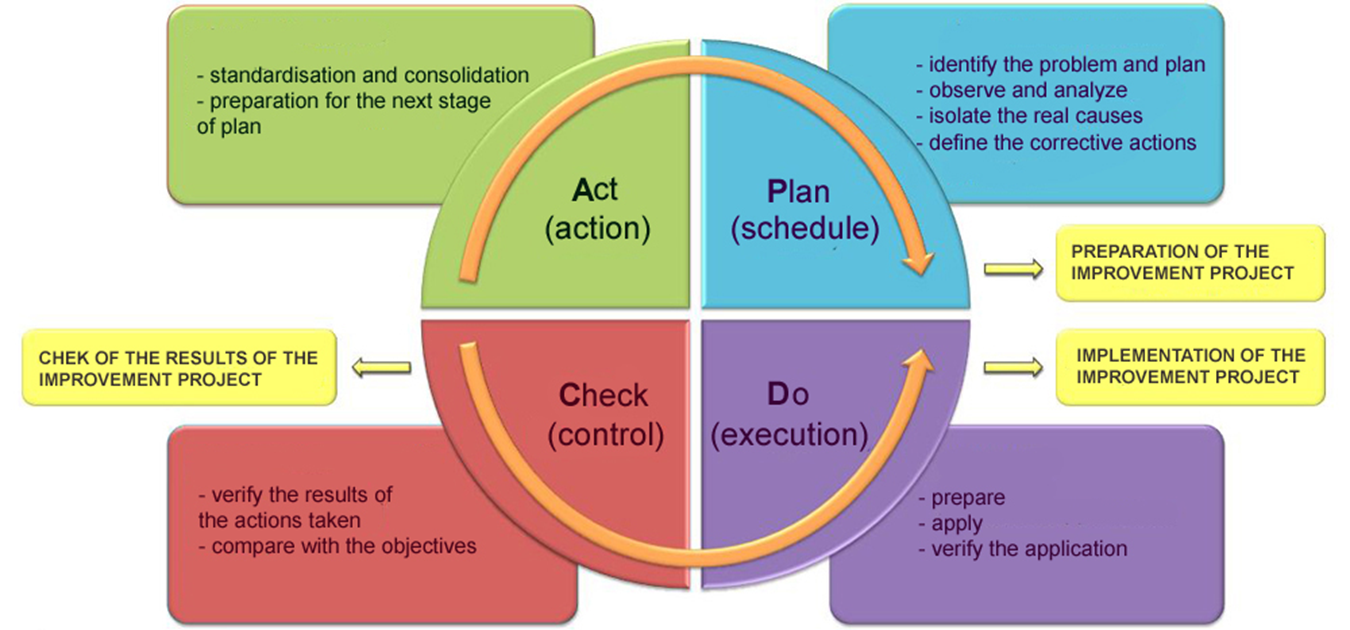
\includegraphics[scale=0.6]{includes/img/pdca.png}
		\caption{Fasi del principio PDCA.}
	\end{figure}

	Infine, il \textit{team\ped{G}} ha individuato dallo standard \textit{ISO/IEC 12207:2008\ped{G}} i processi che ritiene più importanti durante tutto il ciclo di vita del prodotto, al fine di garantire una buona qualità di processo. Per ognuno di essi sono stati individuati obiettivi e metriche coerenti con i livelli di qualità perseguiti.
	
	\subsection{Infrastructure Management Process}
	Questo processo ha lo scopo di fornire, mantenere ed aggiornare l’infrastruttura ed i servizi necessari alla realizzazione del progetto, durante tutto il suo ciclo di vita. Il termine infrastruttura comprende: elementi hardware, software, metodi, strumenti, tecniche e standard impiegati nello sviluppo del prodotto.
	Essa sarà necessaria allo svolgimento del progetto e dovrà essere mantenuta costantemente aggiornata.
	L'utilizzo delle metriche scelte, permetterà di individuare eventuali errori all’interno degli strumenti utilizzati, la cui correzione permetterà di produrre dati corretti e coerenti.
		\subsubsection{Obiettivi}
		Per tutta la durata del progetto, l’infrastruttura impiegata nello sviluppo dovrà raggiungere i seguenti obiettivi:
		\begin{itemize}
			\item ogni procedura riguardante le attività svolte più frequentemente durante lo sviluppo del
			progetto, sarà descritta nel documento \textsc{NormeDiProgetto 1\_0\_0.pdf};
			\item ogni riferimento normativo ed informativo sarà completo di informazioni utili al proprio
			reperimento;
			\item la piattaforma \textit{NetBreakDB} sarà a disposizione di ogni componente del team, in caso di bisogno di accesso ai dati in essa contenuti;
		\end{itemize}
		\subsubsection{Metriche}
			\paragraph{Disponibilità NetBreakDB}
			Indica la percentuale di disponibilità di utilizzo della piattaforma NetBreakDB, rispetto alle richieste di accesso.
			\begin{table}[H]
				\begin{center}
					\begin{tabular}{|c|c|c|}
						\hline
						\textbf{Metodo di calcolo} & \textbf{Range accettazione} & \textbf{Range ottimale} \\
						\hline
						n° acc corr	a pag login/n° tot richieste acc pag login inoltrate & 80-100  & 90-100 \\
						\hline
					\end{tabular}
				\end{center}
				\caption{Disponibilità NetBreakDB}
			\end{table}
	
	\subsection{Project Planning, Assessment \& Control Process}
	Questo processo ha lo scopo di produrre dei piani di sviluppo per il progetto, che comprendano:
	\begin{itemize}
		\item la scelta del modello di ciclo di vita del prodotto;
		\item le descrizioni delle attività e dei compiti da svolgere;
		\item la pianificazione temporale del lavoro e dei costi da sostenere;
		\item l'allocazione di compiti e responsabilità;
		\item le misurazioni per rilevare lo stato del progetto, rispetto alle pianificazioni stilate.
	\end{itemize}
	Durante tutta l’attività di	progetto, sarà fondamentale mantenere aggiornata la pianificazione effettuata, in modo da essere sempre coerente con la situazione attuale. Nel caso in cui, in una fase di lavoro, venissero rilevati dei valori negativi, attraverso l'utilizzo delle metriche scelte Schedule Variance e Budget Variance, occorrerà compensare tali valori entro la fine dell’attività di progetto, al fine di evitare di eccedere le ore di lavoro totali e, di conseguenza, il preventivo dei costi finale indicato nella pianificazione contenuta nel documento \textsc{PianoDiProgetto 1\_0\_0.pdf}.
		\subsubsection{Obiettivi}
		L’intero sviluppo del progetto dovrà seguire la pianificazione prodotta:
		\begin{itemize}
			\item ogni componente dovrà svolgere e portare a termine l'attività assegnatagli, svolgendo tutti i compiti nei quali è stata suddivisa e facendo attenzione a rispettare le scadenze fissate;
			\item il costo necessario allo svolgimento di un'attività non dovrà eccedere la somma
			preventivata.
		\end{itemize}
		\subsubsection{Metriche}
			\paragraph{Schedule Variance}
			Indica se si è o meno in linea con la pianificazione temporale delle attività nella baseline.
			Se si ottiene un valore positivo significa che il team è in anticipo rispetto alla pianificazione, altrimenti significa che si è in ritardo.
			\begin{table}[H]
				\begin{center}
					\begin{tabular}{|c|c|c|}
						\hline
						\textbf{Metodo di calcolo} & \textbf{Range accettazione} & \textbf{Range ottimale} \\
						\hline
						att compl effett - att che dovrebbero esssere compl secondo pianific  & >=0  & >0 \\
						\hline
					\end{tabular}
				\end{center}
				\caption{Schedule Variance}
			\end{table}
		
		\paragraph{Budget Variance}
		Indica se la spesa sostenuta alla data corrente è superiore o inferiore a quella preventivata in sede di pianificazione.
		Un valore positivo indica che si è speso meno di quanto inizialmente previsto, altrimenti significa che si è speso più del preventivo.
		\begin{table}[H]
			\begin{center}
				\begin{tabular}{|c|c|c|}
					\hline
					\textbf{Metodo di calcolo} & \textbf{Range accettazione} & \textbf{Range ottimale} \\
					\hline
					costo pianif per realiz att di progetto alla data corr - costo effett sost alla data corr & >=0  & >0 \\
					\hline
				\end{tabular}
			\end{center}
			\caption{Budget Variance}
		\end{table}
	
	\subsection{Risk Management Process}
	Questo processo ha l'obiettivo di identificare, analizzare, trattare e monitorare in modo continuo i rischi che possono insorgere durante l’intera attività di progetto.
	Il livello di probabilità dei rischi analizzati dovrà essere costantemente monitorato. Nel caso si manifestasse un rischio, a qualiasi livello di pericolosità, il team dovrà attuare le contromisure previste, al fine di mitigare i suoi effetti ed evitare un incremento del livello di pericolosità.
		\subsubsection{Obiettivi}
		Il team dovrà gestire correttamente i rischi:
		\begin{itemize}
			\item all’inizio dell’attività di progetto, verranno individuati i principali fattori di rischio riguardanti l’organizzazione delle attività;
			\item all’inizio di ogni attività, l’analisi dei rischi potrà portare all’individuazione di nuovi specifici rischi per ognuna di esse;
			\item i rischi analizzati che si manifesteranno, verranno trattati secondo le strategie descritte, così da controllarne l'impatto.
		\end{itemize}
		\subsubsection{Metriche}
			\paragraph{Rischi non preventivati}
			Indicatore che evidenzia i rischi non preventivati.
			\begin{table}[H]
				\begin{center}
					\begin{tabular}{|c|c|c|}
						\hline
						\textbf{Metodo di calcolo} & \textbf{Range accettazione} & \textbf{Range ottimale} \\
						\hline
						contatore increm nel mom in cui si manifesta risc non ind in anal dei risc & 0-5  & 0 \\
						\hline
					\end{tabular}
				\end{center}
				\caption{Rischi non preventivati}
			\end{table}
	
	\subsection{System/Software Requirements Analysis Process}
	Questo processo ha lo scopo di creare un insieme di requisiti tecnici, a partire dall'insieme di requisiti individuati dalle fonti, in modo che diventi la linea guida nella progettazione del prodotto.
	Ogni requisito individuato dovrà essere inserito correttamente nella piattaforma NetBreakDB, la quale si occuperà di effettuare il tracciamento delle fonti dalle quali derivano i requisiti, delle modifiche effettuate e della loro implementazione nel prodotto.
		\subsubsection{Obiettivi}
		I requisiti identificati dovranno essere gestiti in modo da raggiungere i seguenti obiettivi:
		\begin{itemize}
			\item per ogni requisito dovrà essere possibile indicare dei test, da effettuare per verificarne il soddisfacimento da parte del prodotto;
			\item nessun requisito dovrà risultare ambiguo;
			\item tutti i requisiti che il prodotto andrà a soddisfare, saranno stati precedentemente approvati dai committenti.
		\end{itemize}
		\subsubsection{Metriche}
			\paragraph{Adempimento requisiti obbligatori}
			Indica la percentuale di requisiti obbligatori soddisfatti dal prodotto.
			\begin{table}[H]
				\begin{center}
					\begin{tabular}{|c|c|c|}
						\hline
						\textbf{Metodo di calcolo} & \textbf{Range accettazione} & \textbf{Range ottimale} \\
						\hline
						n° req obbl sodd/n° req obbl identif & 90-100  & 100 \\
						\hline
					\end{tabular}
				\end{center}
				\caption{Adempimento requisiti obbligatori}
			\end{table}
	
	\subsection{System/Software Architectural Design Process}
	Il processo si pone come obiettivo quello di identificare una corrispondenza fra requisiti di sistema ed elementi del sistema. Nel corso dell’attività di progettazione, sia ad alto livello che di dettaglio, le componenti verranno inserite nella piattaforma NetBreakDB. Essa si occuperà di effettuare i tracciamenti fra le componenti e i requisiti che soddisfano, ed inoltre, il tracciamento tra le relazioni presenti e le varie componenti.
		\subsubsection{Obiettivi}
		Durante lo svolgimento delle attività previste da questo processo, il team punterà a definire
		un’architettura adatta agli scopi del progetto:
		\begin{itemize}
			\item ogni componente progettato come parte del sistema risulterà essere necessario per il funzionamento del prodotto e, quindi, costantemente tracciabile ai requisiti che soddisfa;
			\item il sistema dovrà presentare basso accoppiamento ed alta coesione;
			\item ogni componente dovrà essere progettato puntando su incapsulamento, modularizzazione
			e riuso di codice.
		\end{itemize}
		
		\subsubsection{Metriche}
			\paragraph{Fan In}
			In riferimento ad un modulo software, misura quanti altri moduli lo utilizzano durante la
			loro esecuzione.
			Tale indicazione consente di stabilire il livello di riuso implementato.
			\begin{table}[H]
				\begin{center}
					\begin{tabular}{|c|c|c|}
						\hline
						\textbf{Metodo di calcolo} & \textbf{Range accettazione} & \textbf{Range ottimale} \\
						\hline
						ind num incrementato qnd viene ind mod che dur sua exec chiama mod in ogg & >=0  & >=3 \\
						\hline
					\end{tabular}
				\end{center}
				\caption{Fan In}
			\end{table}
			
			\paragraph{Fan Out}
			In riferimento ad un modulo software, misura quanti moduli vengono utilizzati durante la
			sua esecuzione.
			Tale indicazione consente di stabilire il livello di accoppiamento implementato.
			\begin{table}[H]
				\begin{center}
					\begin{tabular}{|c|c|c|}
						\hline
						\textbf{Metodo di calcolo} & \textbf{Range accettazione} & \textbf{Range ottimale} \\
						\hline
						ind num incrementato qnd viene indiv modulo util da mod in ogg durante sua exec & 0-5  & 0-1 \\
						\hline
					\end{tabular}
				\end{center}
				\caption{Fan Out}
			\end{table}
			
	
	\subsection{Software Architectural Design Process}
	Lo scopo del processo è fornire una progettazione di minimo del prodotto che andrà a soddisfare i requisiti individuati.
	Tutte le attività presenti in questo processo portano alla produzione del documento Specifica Tecnica.
		\subsubsection{Obiettivi}
			\begin{itemize}
				\item fornire un'architettura ad alto livello del prodotto software, in grado di soddisfare i requisiti individuati;
				\item definire le interfacce interne ed esterne per ogni componente individuato;
				\item progettare uno schema ad alto livello del database. 
			\end{itemize}

		\subsubsection{Metriche}
			\paragraph{Numero di interfacce??}
			Indica il numero di interfacce definite.
			\begin{table}[H]
				\begin{center}
					\begin{tabular}{|c|c|c|}
						\hline
						\textbf{Metodo di calcolo} & \textbf{Range accettazione} & \textbf{Range ottimale} \\
						\hline
						formula & xx  & yy \\
						\hline
					\end{tabular}
				\end{center}
				\caption{Numero di interfacce}
			\end{table}
		
			\paragraph{Altre metriche??}
	
	\subsection{Software Detailed Design Process}
	Lo scopo del processo è fornire una progettazione dettagliata del prodotto che andrà ad implementare i requisiti individuati.
	Sarà necessario effettuare un’analisi dettagliata delle componenti individuate durante l'attività di progettazione
	architetturale, suddividendole in unità che siano facilmente codificabili e testabili.
		\subsubsection{Obiettivi}
		Le attività svolte dovranno raggiungere i seguenti obiettivi:
		\begin{itemize}
			\item il livello di dettaglio della progettazione dovrà indicare tutti i metodi, con i relativi parametri e campi dati, forniti da ciascuna classe;
			\item la struttura a basso livello dell’architettura e le relazioni fra le varie unità software concepite saranno esposte nel documento di Definizione di Prodotto, il quale definirà esattamente cosa implementare;
		\end{itemize}
		
		\subsubsection{Metriche}
			\paragraph{Numero di metodi per classe}
			Indica il numero di metodi definiti in una classe.
			Un valore molto alto potrebbe indicare una
			non buona decomposizione delle funzionalità a livello logico.
			\begin{table}[H]
				\begin{center}
					\begin{tabular}{|c|c|c|}
						\hline
						\textbf{Metodo di calcolo} & \textbf{Range accettazione} & \textbf{Range ottimale} \\
						\hline
						formula & 1-10  & 1-5 \\
						\hline
					\end{tabular}
				\end{center}
				\caption{Numero di metodi per classe}
			\end{table}
		
			\paragraph{Numero di parametri per metodo}
			Indica il numero di parametri passati ad un metodo.
			Un valore molto alto potrebbe indicare un'eccessiva complessità del metodo, il quale potrebbe non essere sufficientemente scomposto in sotto-metodi.
			\begin{table}[H]
				\begin{center}
					\begin{tabular}{|c|c|c|}
						\hline
						\textbf{Metodo di calcolo} & \textbf{Range accettazione} & \textbf{Range ottimale} \\
						\hline
						formula & 0-8  & 0-4 \\
						\hline
					\end{tabular}
				\end{center}
				\caption{Numero di parametri per metodo}
			\end{table}
		
			\paragraph{Numero di attributi per classe}
			Indica il numero di attributi di una classe.
			Un valore molto alto potrebbe suggerire la necessità di suddividere tale classe in più classi differenti correlate tra loro.
			\begin{table}[H]
				\begin{center}
					\begin{tabular}{|c|c|c|}
						\hline
						\textbf{Metodo di calcolo} & \textbf{Range accettazione} & \textbf{Range ottimale} \\
						\hline
						formula & 0-12  & 2-8 \\
						\hline
					\end{tabular}
				\end{center}
				\caption{Numero di attributi per classe}
			\end{table}
			
	\subsection{Software Construction Process}
	Questo processo definisce le principali attività volte alla produzione di unità software eseguibili, che
	rispettino quanto prodotto durante la progettazione.
	Nell’attività di codifica, il \textit{\Progr} dovrà semplicemente attenersi a quanto indicato nel documento Definizione di Prodotto. Inoltre, sarà necessario procedere con la codifica dei test individuati in sede di progettazione, al fine di verificare il corretto funzionamento delle varie unità prodotte.
		
		\subsubsection{Obiettivi}
		Affinchè le unità software prodotte risultino di qualità, il team ha individuato i seguenti obiettivi:
		\begin{itemize}
			\item l’implementazione delle classi e dei metodi definiti in progettazione dovrà produrre codice a bassa complessità, in modo da facilitare l'attività di test;
			\item l’uso di costrutti e tecniche che creano sdoppiamenti del flusso di esecuzione verrà attuato solo se strettamente necessario;
			\item il codice prodotto dovrà risultare facilmente manutenibile;
			\item il codice prodotto risulterà privo di elementi inutilizzati.
		\end{itemize}
		
		\subsubsection{Metriche}
			\paragraph{Complessità Ciclomatica}
			Indica la complessità di funzioni, moduli, metodi o classi di un programma, misurando il numero
			di cammini linearmente indipendenti attraverso il grafo di controllo di flusso.
			Alti valori di complessità ciclomatica implicano una ridotta manutenibilità del codice; viceversa, bassi valori potrebbero determinare una scarsa efficienza dei metodi.
			\begin{table}[H]
				\begin{center}
					\begin{tabular}{|c|c|c|}
						\hline
						\textbf{Metodo di calcolo} & \textbf{Range accettazione} & \textbf{Range ottimale} \\
						\hline
						n° archi - n° nodi + 2 & xx  & yy \\
						\hline
					\end{tabular}
				\end{center}
				\caption{Complessità Ciclomatica}
			\end{table}
			
			\paragraph{Numero di livelli di annidamento}
			Indica il numero di funzioni o procedure chiamate all’interno di un metodo.
			Un valore elevato implica un’alta complessità ed un basso livello di astrazione del codice.
			\begin{table}[H]
				\begin{center}
					\begin{tabular}{|c|c|c|}
						\hline
						\textbf{Metodo di calcolo} & \textbf{Range accettazione} & \textbf{Range ottimale} \\
						\hline
						ind num ind num chiam a funz o proc pres in un metodo & 1-8  & 1-4 \\
						\hline
					\end{tabular}
				\end{center}
				\caption{Numero di livelli di annidamento}
			\end{table}
		
			\paragraph{Linee di commento}
			Indica la percentuale di linee di commento presenti all’interno del codice sorgente; la loro presenza
			permette una più semplice comprensione ed un maggior livello di manutenibilità di quanto
			prodotto.
			\begin{table}[H]
				\begin{center}
					\begin{tabular}{|c|c|c|}
						\hline
						\textbf{Metodo di calcolo} & \textbf{Range accettazione} & \textbf{Range ottimale} \\
						\hline
						num linee commento presenti nel
						codice/SLOC prodotte & >=20  & >=35 \\
						\hline
					\end{tabular}
				\end{center}
				\caption{Linee di commento}
			\end{table}
	
	\subsection{System/Software Integration Process (6.4.5 - 7.1.6)}
	
	\subsection{System/Software Qualification Testing Process (6.4.6 - 7.1.7)}
	
	\subsection{Software Documentation Management Process (7.2.1)}
	
	\subsection{Software Verification Process (7.2.4)}
	
\newpage
\section{Resoconto delle attività di verifica}

	\subsection{Dettaglio delle verifiche tramite analisi}
	
	\subsubsection{Documenti}
	
	\paragraph{Fase di Analisi}
	
	



\end{document}